\chapter{Projektafgrænsninger}
Dette kapitel beskriver projektets afgrænsninger og hvilke arbejdsopgaver der blevet frasorteres i udviklingsfasen. Afgrænsninger kan både være til der er helt undladt i projektet, eller bestemte faktorer der har begrænset udvikling af vise dele i systemet. 

\section{Sikkerhedskontrol} \label{title:sikkerhedskontrol}
Fra projekts start i forprojektet lå der et ønske fra kundens side omkring en sikkerhedskontrol ved konditioneringsbehandlingen. Fra kundens side bestod ønsket i at kontrollere kredsløbet på patienten, der modtog konditioneringsbehandling. Ønsket lød på at bruge et pulsoximeter som sikkerhedskontrol. Det færdige produkt skulle ved hjælp af et pulsoximeter tjekket patients saturation og puls og ud fra threshold værdier vurdere om patienten kunne tåle behandlingen. De tænkte cases, hvor sikkerhedskontrollen skulle afbryde behandlingen, var ved patienter med dårligt kredsløb, som under behandlingen udvikler koldbrand i den afklemte ekstremitet. Problematikken ved at bruge et pulsoximeter som sikkerhedskontrol ligger i teknikken bag pulsoximeteri. 

Pulsoximeteri måler variationer i det pulserende blod ved at detektere ændringerne i absorption af lys fra to eller flere lyskilder med forskellige bølgelængder. Når væv belyses kan absorptionsgrundlaget opdeles i fire dele (Se figur \ref{fig:opticTissue})
\begin{figure}[H]
	\centering
	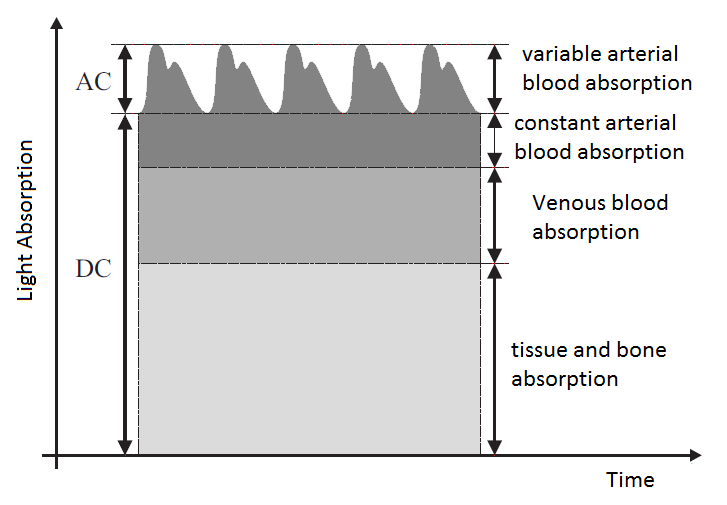
\includegraphics[width = 0.7\textwidth]{billeder/opticTissue.png}
	\caption{Oversigt over absorption af lys i væv}\label{fig:opticTissue}
\end{figure}

I pulsoximeteri filtreres alt DC væk, dvs absorption fra venøst blod, den konstante mængde af arterielt blod og alt andet væv og der kigges kun på signal fra det pulserende arterielle blod. For at måle saturationen udregnes forskellen på absorption ved \textit{pulstop} og \textit{pulsbund}. Disse absorption kan ved hjælp af de molar extinction koefficienter for hhv. oxyhæmoglobin og deoxyhæmoglobin og afstanden mellem lyskilde og modtager omregnes til relative koncentrations ændring i hhv. oxyhæmoglobin og deoxyhæmoglobin. Disse relative koncentration ændringer kan så omsættes til saturation via formlen \ref{eq:satequation}
\begin{equation}
	SaO_2 = \frac{\Delta[HbO_2]}{\Delta[HbO_2]+\Delta[HHb]}
	\label{eq:satequation}
\end{equation}

På grund af pulsoximeteri kun giver oplysninger omkring pulserende arteriel blod og at iltforsyningen af væv foregår via kapillærerne, mangler der information om kredsløbet i kapillærerne. På den måde giver pulsoximeteri en indikator for respirationen og for hvor iskemisk vævet er. Sikkerhedskontrollen skulle kontrollere om iltreserven i armen nået op på et tilstrækkeligt niveau efter hver afklemning, men pga det pulserende signal fra dette arterielle blod er meget små signaler, er et pulsoximeter udviklet til at detektere meget små signal. Derfor kan selv en person med dårlig kredsløb få målt en puls og saturation uden at vide om hans væv tager skade af konditioneringsbehandlingen. 

Denne problemstilling blev opdaget forholdsvis hurtigt i projektforløbet og kunden blev orienteret omkring problemstillingen. Det blev derfor bestemt at projektet skulle afgrænses i forbindelse med sikkerhedskontrollen. Der er gjort plads i udviklingsdokumentation til at implementering af en anden form for sikkerhedskontrol. For at få underbygget påstanden omkring pulsoximeteri og sikkerhedskontrol, har projektgruppen været i kontakt med Troels Johansen fra lungemedicinsk afsnit på AUH (Se afsnit \ref{title:samarbejdspartnere} omkring samarbejdspartnere og mødereferater \fixme{Reference til mødereferat med Troels Johansen}). Troels kunne kun bekræfte påstanden omkring at pulsoximeteri som være ugyldig til sikkerhedskontrol, og så istedet muligheder i NIRS(Se afsnit \ref{title:nirs} i perspektivering) eller at bruge pulsoximeteri som kontrol af om afklemningen var tilstrækkeligt. 

\section{MR kompatibilitet}
I forbindelse med forprojektet var et ønskescenarie fra kunden side at apparatet der skulle udviklings til at udfører konditionering skulle kunne gå i en MR-scanner. Dette var et ønske fordi perkonditionering, hvis det køres i fx 4 cyklusser af 5 minutter, vil tage længere til at gennemfører, end den tid det tager at kører til hospitalet. Proceduren for patient der mistænkes for have apopleksi er at få dem i MR scanneren så hurtigt så muligt, og derfor kan man i nogle tilfælde være nød til at afbryde konditioneringsbehandlingen og der kan stilles spørgsmålstegn ved den gavnlige effekt. Det blev meget hurtigt bestemt af projektet måtte afgrænse sig fra at lave apparatet MR kompatibel, da dette ville stille alt for høje krav til produktets komponenter.

\section{Signal behandling}

\section{Seagull samarbejde}
I begyndelse af projektet blev der igennem kunden etableret et sammen arbejdet med en dansk virksomhed, som skulle fungere som talerør til en kinesisk blodtryksapparat producent (Se afsnit \ref{title:samarbejdspartnere} omkring samarbejdspartnere). Tanken bag samarbejdet var et den kinesiske virksomhed skulle kunne bestå med komponenter og teknisks sparringen. Grunden til den danske virksomhed var med som mellemmand var et ønske fra deres side, da den kinesiske virksomhed var deres kontakt. Et andet argument for at det skulle være sammen arbejde med virksomheder var et ønskede fra kunden side omkring produktet skulle lige sig tæt opad Seagulls apparatet. 

Men efter flere forgæves forsøg for at kommunikere og få information ud af den kinesisk virksomhed blevet det opgivet at produktet skulle ligge sig op af deres apparater. Det forgæves samarbejde betød også at arbejdet med en blodtryksalgoritme måtte foretages på egen hånd af projektgruppen selv. 

\section{Prototypen}